\clearpage
\section{Results}
\label{sec:results}

% TODO introduce results & reiterate RQ





% table (mean, quantiles) of the optimal X-minute city metric
Table \ref{tab:optimal_x_minute_city_metric} shows the mean, as well as, the 25\%, 50\% and 75\% quantiles of the optimal X-minute city disregarding the cost for each scenario.

\begin{table}
  \caption{Optimal X-minute city metric over all hexagons disregarding cost}
  \label{tab:optimal_x_minute_city_metric}
  \begin{center}
    \begin{tabular}{|l|r|r|r|r|}
    \hline
    scenario & mean & 25\% & 50\% & 75\% \\
    \hline
    bicycle & 11.82 & 7.00 & 10.00 & 15.00 \\
    \hline
    bicycle_public_transport & 11.09 & 7.00 & 10.00 & 14.00 \\
    \hline
    car & 3.21 & 2.00 & 3.00 & 4.00 \\
    \hline
    public_transport & 12.62 & 9.00 & 12.00 & 15.00 \\
    \hline
    walking & 14.09 & 9.00 & 12.00 & 17.00 \\
    \hline
    \end{tabular}
  \end{center}
\end{table}


We can make a few interesting observations from this table:
First, adding public transport to walking improves the average optimal time it takes to reach all categories by 1 minute and 28 seconds.
From the quantiles we can see that this improvement is not evenly distributed, but only applies to the 25\% worst hexagons.
Specifically we see no improvement from walking to public transport in the 25\% and 50\% quantiles, but a 2-minute improvement in the 75\% quantile.

Similarly, adding public transport to bicycle sharing improves the average optimal time it takes to reach all categories by 43 seconds.
Again, this improvement is not evenly distributed, but only applies to the 25\% worst hexagons.
Specifically we see no improvement from bicycle sharing to public transport in the 25\% and 50\% quantiles, but a 1-minute improvement in the 75\% quantile.
While there is an improvement in the mean and 75\% quantile, it is not as large as the improvement from walking to public transport.

% visualization of the distribution of the optimal X-minute city metric
We can observe a similar pattern when visualizing the distribution of the optimal X-minute city metric in Figure \ref{fig:optimal_x_minute_city_metric}.

\begin{figure}
  \begin{center}
    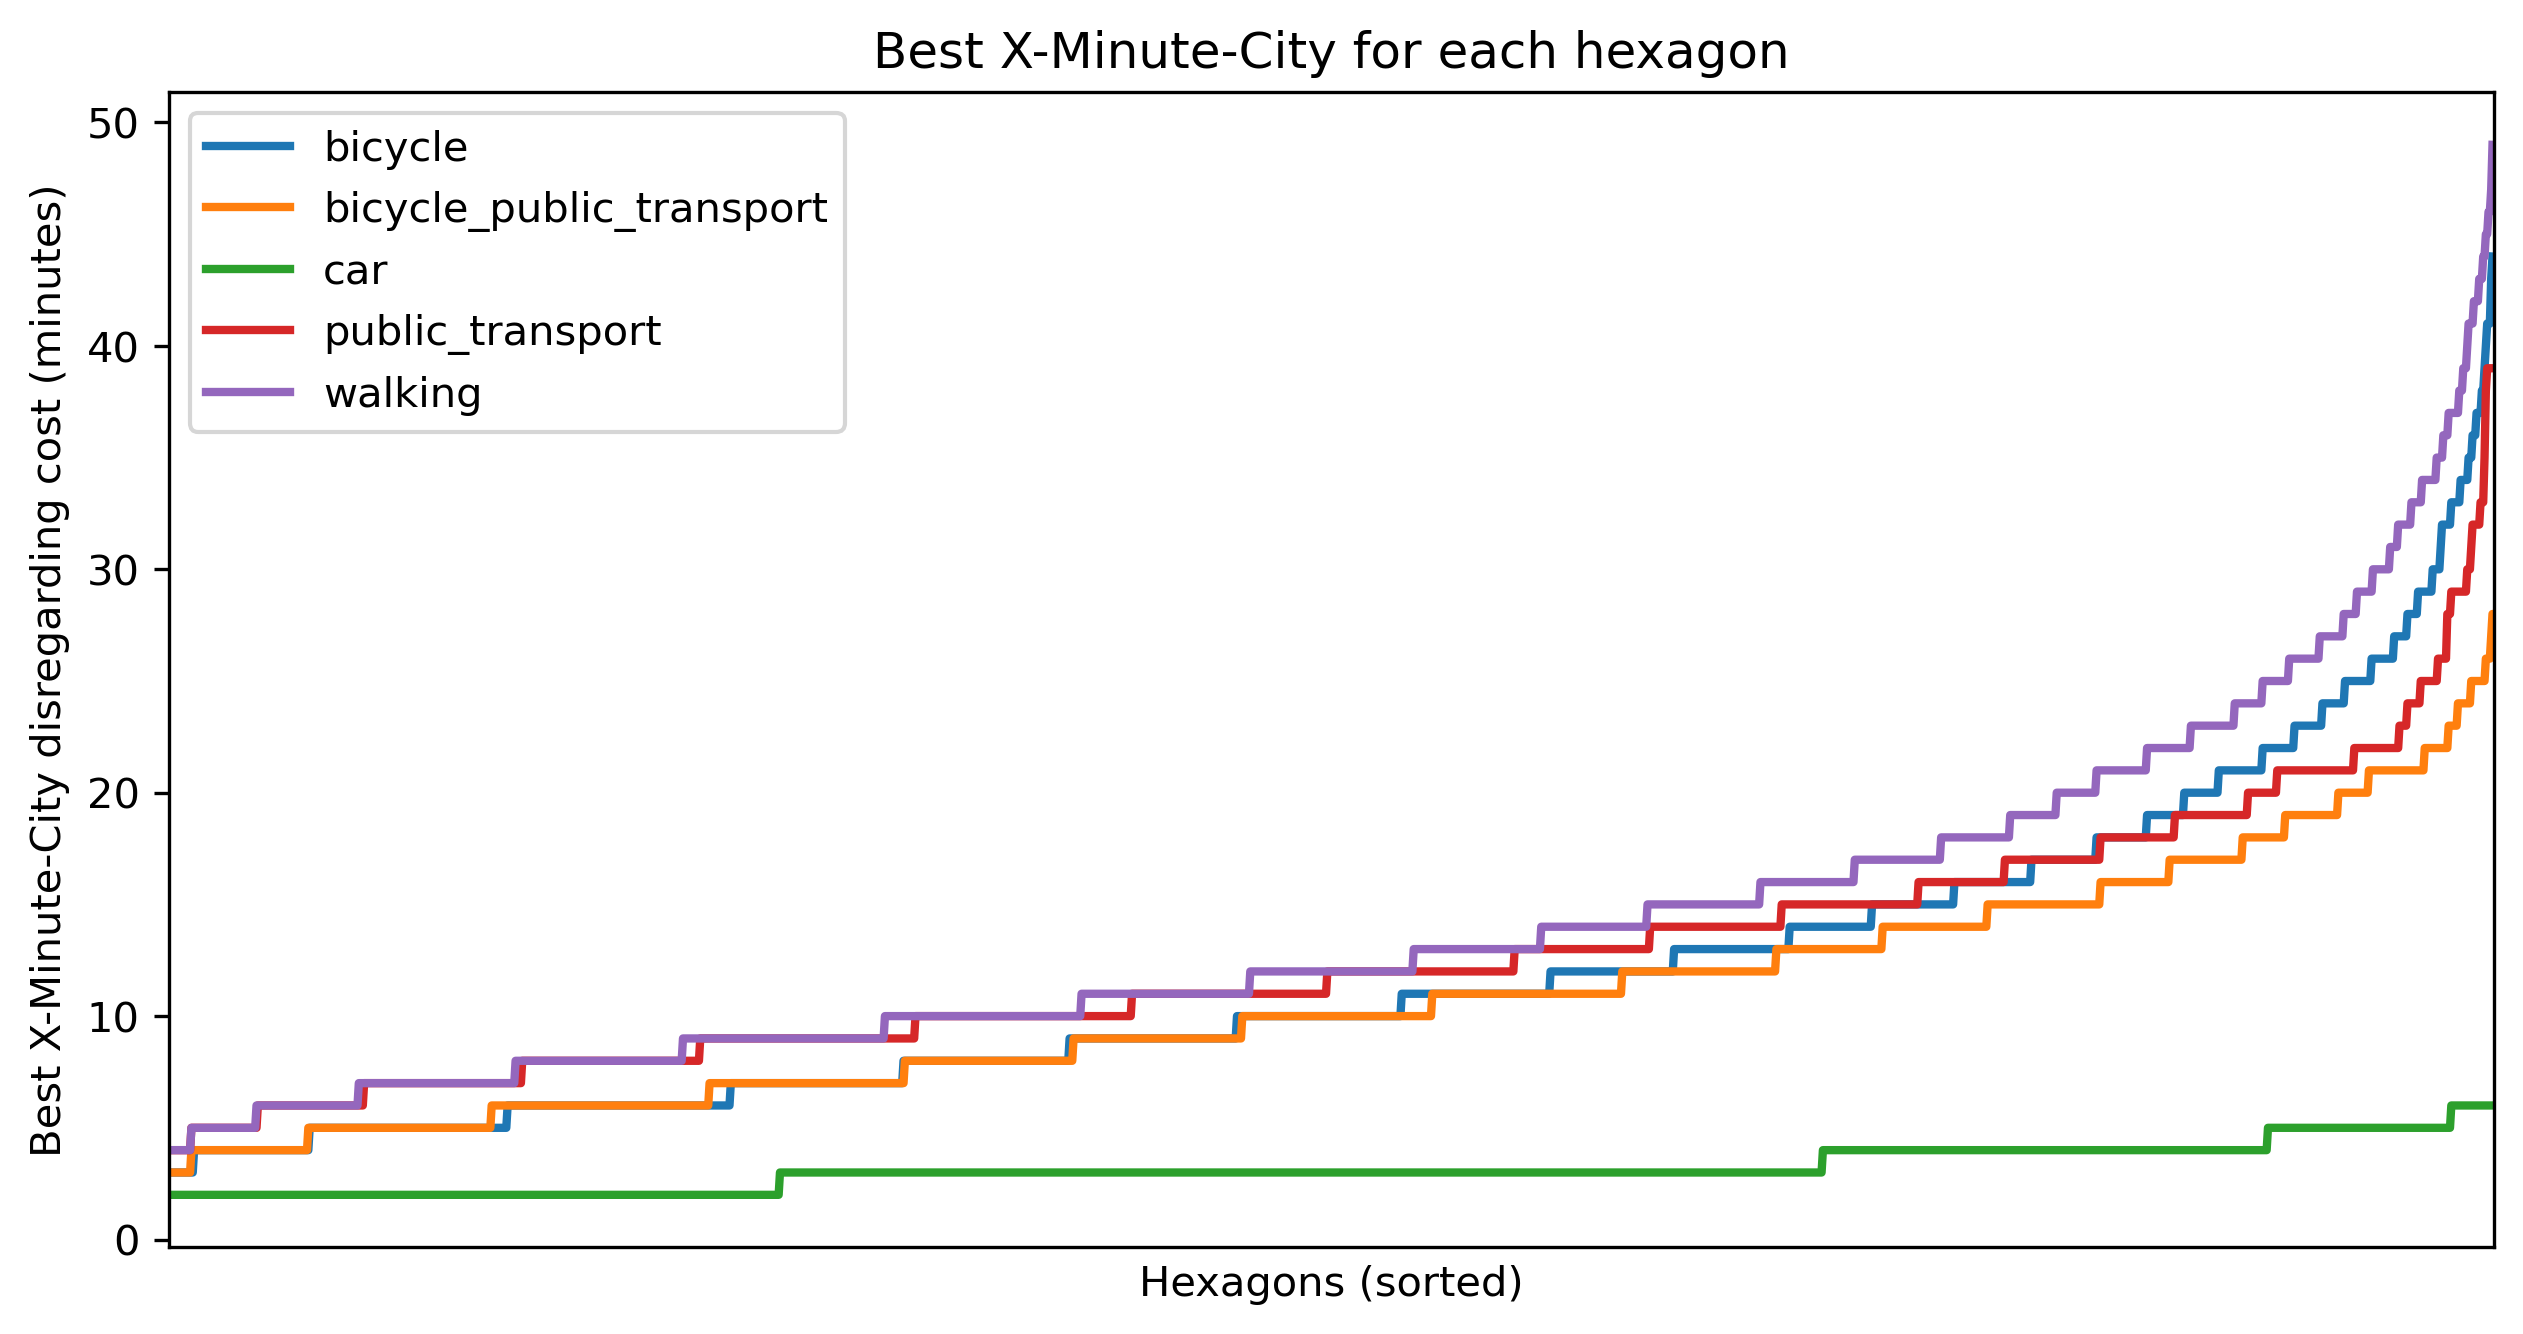
\includegraphics[width=0.65\textwidth]{Figures/results/best_x_minute_city}
  \end{center}
  \caption{Distribution of optimal x-minute city metric}\label{fig:optimal_x_minute_city_metric}
\end{figure}


As we can see initially (for the most accessible hexagons) public transport and walking are the same, but as we move to less accessible hexagons public transport becomes better.
In addition, the public transport scenario is worse than the pure bicycle sharing scenario, but is able to catch up to it and even overtake it as we move to less accessible hexagons.

The same pattern can be observed when comparing the bicycle sharing scenario to the combined scenario of bicycle sharing and public transport.
Initially, the combined scenario is the same as the bicycle sharing scenario, but as we move to less accessible hexagons the combined scenario becomes better.

Generally, we see that adding public transport is able to flatten the drastic increase of the optimal X-minute city metric at the end of the distribution.

% table (mean, quantiles) of required cost
Table \ref{tab:required_cost} shows the mean, the 25\%, 50\% and 75\% quantiles and the max of the cost that are required to achieve the optimal value for the X-minute city.

\begin{table}
  \caption{Required cost for optimal over all hexagons}
  \label{tab:required_cost}
  \begin{center}
    \begin{tabular}{|l|r|r|r|r|r|}
    \hline
    scenario & mean & 25\% & 50\% & 75\% & max \\
    \hline
    bicycle & 0.50 & 0.00 & 0.00 & 1.00 & 1.00 \\
    \hline
    bicycle_public_transport & 0.94 & 0.00 & 1.00 & 1.00 & 4.20 \\
    \hline
    car & 0.37 & 0.19 & 0.38 & 0.38 & 1.33 \\
    \hline
    public_transport & 0.70 & 0.00 & 0.00 & 2.20 & 3.20 \\
    \hline
    walking & 0.00 & 0.00 & 0.00 & 0.00 & 0.00 \\
    \hline
    \end{tabular}
  \end{center}
\end{table}

We can immediately see that there is no cost for hexagons at the 25\% and 50\% quantile when using public transport.
This means that for those hexagons, no public transport is actually used, as it will not yield any improvements compared to walking.
Looking at the 75\% quantile and the maximum of the required cost for an optimal x-minute city metric for public transport, we see that the benefits we observed earlier come at a cost.

Similarly, comparing bicycle sharing to the combined scenario of bicycle sharing and public transport, we see that the maximum required cost is 4.20€ for the combined scenario, compared to 1.00€ for the bicycle sharing scenario.
This again shows that the benefits of adding public transport come at a cost.

We can make the same observation with more granularity when looking at the distribution of the required cost in Figure \ref{fig:maximum_required_cost_for_x_minute_city}.

\begin{figure}
  \begin{center}
    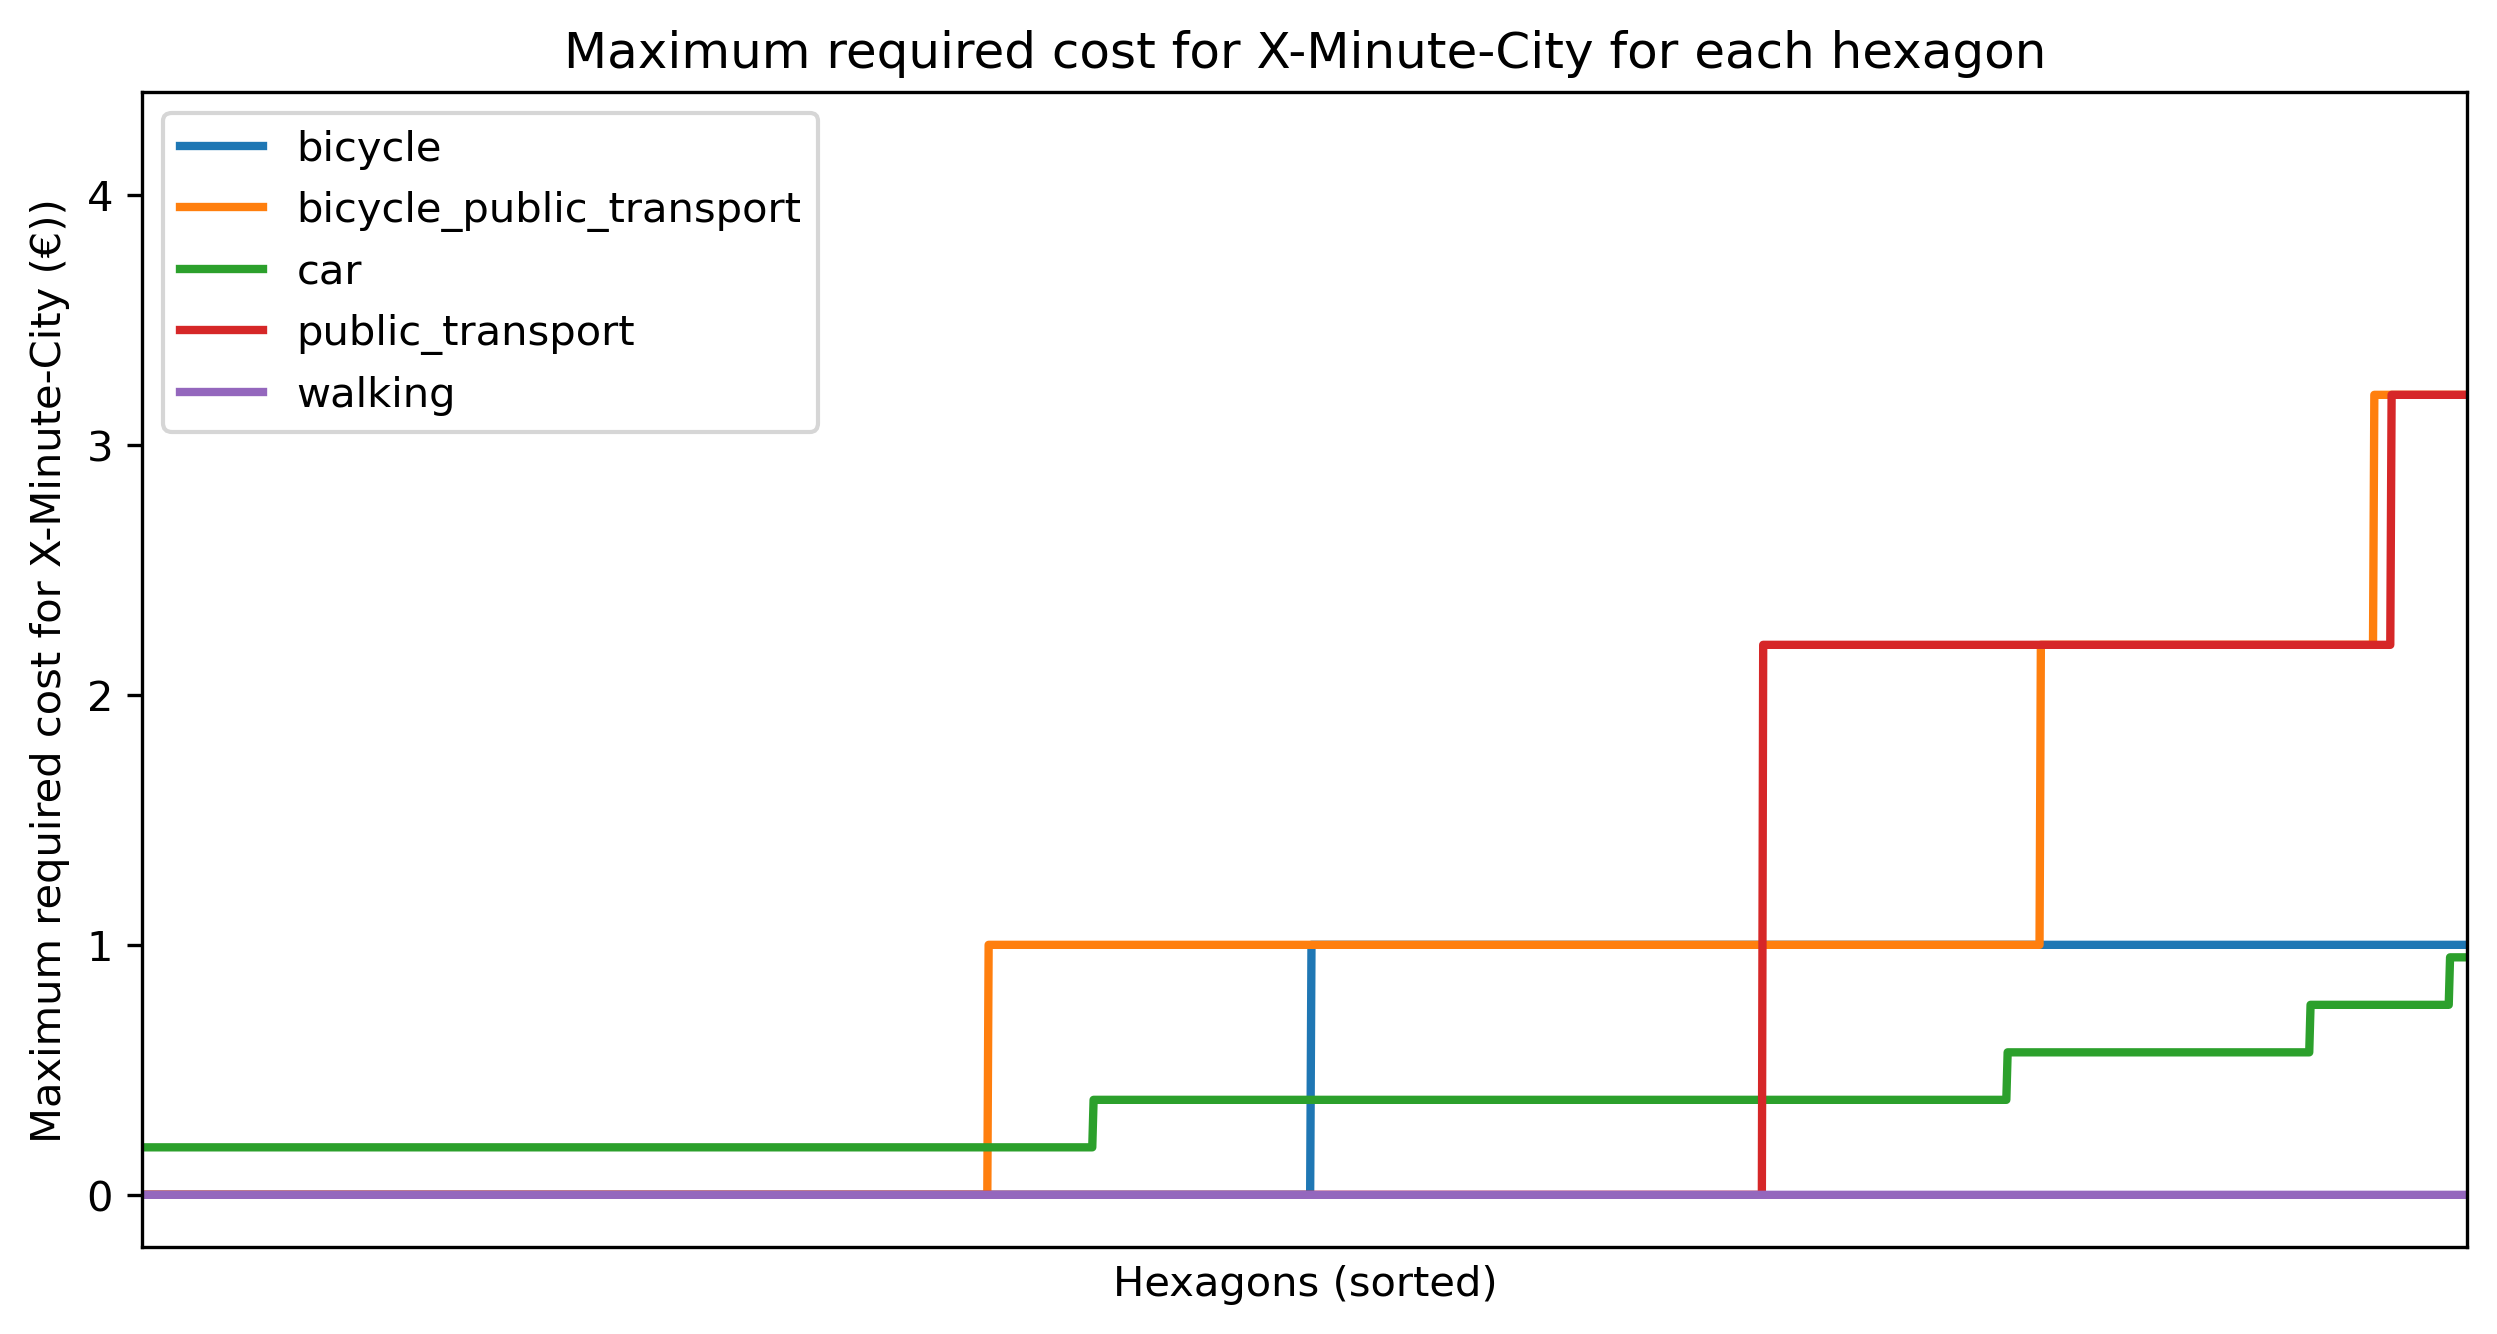
\includegraphics[width=0.65\textwidth]{Figures/results/maximum_required_cost_for_x_minute_city}
  \end{center}
  \caption{Maximum required cost for optimal x-minute city metric}
  \label{fig:maximum_required_cost_for_x_minute_city}
\end{figure}

One interesting remark is that the maximum required cost for the bicycle sharing scenario is 1.00€, which implies that it is never necessary to use a bicycle more than 15 minutes to reach all categories.
This shows that the City of Cologne is already a 15-minute city in terms of cycling at the locations where bicycle sharing is available.
